\documentclass[a4paper, 11pt, spanish, oneside]{book}

\newcommand{\plogo}{\fbox{$\mathcal{PL}$}} 
\usepackage{amsmath}
\usepackage[utf8]{inputenc} 
\usepackage[T1]{fontenc} 
\usepackage{enumitem}
\usepackage{graphicx}
\usepackage{fancyhdr}
\usepackage{hyperref}
\pagestyle{fancy}


\begin{document} 

\begin{titlepage} 

	\centering 
	
	\scshape 
	
	\vspace*{\baselineskip} 
	
	
	
	\rule{\textwidth}{1.6pt}\vspace*{-\baselineskip}\vspace*{2pt} 
	\rule{\textwidth}{0.4pt} 
	
	\vspace{0.75\baselineskip} 
	
	{\LARGE Proyecto: Cobertura de vértices mínima con colonia de hormigas}	
	\vspace{0.75\baselineskip} 
	
	\rule{\textwidth}{0.4pt}\vspace*{-\baselineskip}\vspace{3.2pt}
	\rule{\textwidth}{1.6pt} 
	
	\vspace{2\baselineskip} 
	

	Heurísticas de Optimización Combinatoria
	
	\vspace*{3\baselineskip} 
	
	
	Alumna:
	
	\vspace{0.5\baselineskip} 
	
	{\scshape\Large Karla Adriana Esquivel Guzmán \\} 
	\vspace{0.5\baselineskip} 
	\includegraphics[scale=0.20]{/home/karly/Desktop/1.png}
	\vfill
	\textit{UNIVERSIDAD NACIONAL AUTONOMA DE MEXICO} 
	
	
	
	
	
	
	\vspace{0.3\baselineskip} 
	
	16/Diciembre/2018 
	
	 

\end{titlepage}
\newpage
Como segundo proyecto del curso elegí hacer una implementación para encontrar \textbf{la cobertura de vértices mínima con una colonia de hormigas} el lenguaje de programación que se utilizó para este proyecto es \textbf{Go} y para generar las gráficas se utilizó \textbf{SVG}.

\begin{itemize}
 \item\textbf{Problema:} Encontrar una cubierta en una gráfica G con el menor número de vértices posible.
 \item\textbf{Go:} Nuevamente utilicé el lenguaje de programación Go para adquirir más experiencia con este lenguaje.
 \item\textbf{SVG:} SVG es un formato gráfico basado en XML, decidí gráficar con SVG porque es muy fácil de utilizar y dibuja de manera bonita las gráficas.
 \item\textbf{Implementación:} Es una implementación sencilla, se hizo con base en el paper \textbf{An Ant Colony Optimization Algorithm for the Minimum Weight Vertex Cover Problem}, la dificultad principal fue entender como funcionaban los dos tipos de feromonas, puesto que hay una global y una local, una vez entendido lo anterior la implementación del algoritmo no tuvo gran dificultad.
 \item\textbf{Estructuras}:\\
 Esta estructura reprenta un vértice, cada vértice debe tener un valor de feromona inicial y un valor de la feromona que se modificará con cada iteración.
 \begin{verbatim}
  type Vertex struct {
    index int
    pheromone_init float64
    pheromone float64
  }
 \end{verbatim}
 Esta estructura representa una arista, cada arista tiene dos valores los cuales son los índices de los vértices en los que incide, así como también debe tener un peso inicial.
 \begin{verbatim}
  type Edge struct {
    v1_index int
    v2_index int
    weight float64
 }
 \end{verbatim}
 \newpage
 Esta estructura representa una gráfica, contiene un \textbf{slice} de veritces, que es un aputnador para que todas las gráficas que se definan para las hormigas hagan referencia al mismo \textbf{slice}.
 \begin{verbatim}
  type Graph struct {
    vertexes *[]Vertex
    edges *[]Edge
    full *[]Edge
  }
 \end{verbatim}
 Esta estructura representa una hormiga, la cual tiene como parámetros un índice index, el cuál sirve como un identificador para la hormiga, tenemos también el apuntador a una gráfica graph, un apuntador a un generador aleatorio random(genera números aleatoriamente), solution es un \textbf{slice} de enteros para guardar las soluciones de cada hormiga. Un parámetro q0 que es un valor fijo definido para experimentación, tenemos evaporation\_rate esté parametro se utiliza para ajustar la actualización global y pheromone\_adjust para ajusta la feromona local, por último tenemos el parámetro beta que es un valor fijo definido desde el inicio para experimentación, sirve para ``rankear'' (darle cierto peso) a la feromona.
 
 \begin{verbatim}
  type Ant struct {
    index int
    graph *Graph
    random *rand.Rand
    solution *[]int
    q0 float64
    evaporation_rate float64
    pheromone_adjust float64
    beta float64
   }

 \end{verbatim}
 \newpage
 \item\textbf{Funciones:}\\
 Utilizando la fórmula especificada en el paper, esta función hace la actualización de la feromona local después de que la hormiga se posiciona sobre el vértice.
 \begin{verbatim}
func (a Ant) ActualizaFeromonaLocalmente(indexVertex int){
pheromone0 := (*(*a.graph).vertexes)[indexVertex].pheromone_init
pheromonei := (*(*a.graph).vertexes)[indexVertex].pheromone
(*(*a.graph).vertexes)[indexVertex].pheromone = 
((1-a.pheromone_adjust)*pheromonei)+(a.pheromone_adjust*pheromone0
 \end{verbatim}
 Esta función simula un ``paso'' de la hormiga, es decir a que nodo será el siguiente al que avanzará, viene explicitamente comentada cada una de las lineas en el código.
 \begin{verbatim}
func (a Ant) Paso() {
    q := a.random.Float64()
    rnvalues := a.GetVertexesRNValue() 
    sumrnValues := 0.0
    maxrnValue := 0.0
    indexmaxrnValue := -1 
    count := 0;
    for count < len(rnvalues) {
        if maxrnValue <= rnvalues[count] {
            maxrnValue = rnvalues[count]
            indexmaxrnValue = count
        }
        sumrnValues = sumrnValues + rnvalues[count]
        count = count+1
    }
    if q < a.q0{
    [indexmaxrnValue].pheromone)
    a.AgregaASolucion(indexmaxrnValue)
    a.ActualizaFeromonaLocalmente(indexmaxrnValue)
    (*a.graph).FullEdgesTo0ForVertex(indexmaxrnValue)
    [indexmaxrnValue].pheromone)
        
    
    }else{
        dioPaso := false
        for dioPaso != true{
            randomIndex := rand.Intn(len(rnvalues))
            vertice
            indexProb := (rnvalues[randomIndex]/sumrnValues)
            randonNumber := a.random.Float64()
            indexProb, randonNumber)
            if randonNumber <= indexProb{
                a.AgregaASolucion(randomIndex)
                a.ActualizaFeromonaLocalmente(randomIndex)
                (*a.graph).FullEdgesTo0ForVertex(randomIndex)
                dioPaso = true
            }
         }
     }
}  
 \end{verbatim}
 
 Esta función sirve para determinar si la hormiga puede continuar avanzando en las aristas, si estás tienen un valor distinto de 0.
 \begin{verbatim}
func (a Ant) PuedeDarUnPaso() bool {
    peso := (*a.graph).FullWeight()
    if peso != 0{
        return true
    }else{
        return false
    }
}
 \end{verbatim}
 Esta función es la encargada de calcular el valor RN de cada uno de los vértices.
 \begin{center}
 \begin{verbatim}
  func (a Ant) GetVertexesRNValue() []float64 {
    numVertex := len((*(*a.graph).vertexes))
    rnvalues := make([]float64, numVertex)
    count := 0;
    for count < numVertex {
        indexVertex := (*(*a.graph).vertexes)[count].index
        pheromoneVertex := (*(*a.graph).vertexes)[count].pheromone
        weightVertex := (*a.graph).FullWeightOfVertex(indexVertex)
        rnvalues[indexVertex] = pheromoneVertex*weightVertex
        indexVertex,pheromoneVertex,weightVertex, rnvalues[indexVertex])
        count = count+1
    }
    return rnvalues
 }
 \end{verbatim}
 \end{center}
 
 Ahora explicaré en esta parte la función main que es la más importante de todas, porque se inicializa la gráfica y es en dónde está definida la estructura del algoritmo ACO tal y como está definido en el paper ya mencionado, en el código viene comentado lo que hace cada parte del código.
 
 \begin{verbatim}
  func main() {
    data, err := ioutil.ReadFile("g.txt")
    if err != nil {
        fmt.Println("File reading error", err)
        return
    }
    rows := strings.Split(string(data), "\n")
    numOfVertexes, _ := strconv.Atoi(rows[0])
    vertexesG := make([]Vertex, numOfVertexes)
    count := 0;
    for count < numOfVertexes {
        vertexesG[count] = Vertex{count, 0.1, 0.2}
        count = count + 1
    }

    numOfEdges := len(rows)-2
    edgesG := make([]Edge, numOfEdges)
    count = 0;
    for count < numOfEdges {
        vertIndx := strings.Split(rows[count+1], ",")  
        vertex1, _ := strconv.Atoi(vertIndx[0])
        vertex2, _ := strconv.Atoi(vertIndx[1])
        edgesG[count] = Edge{vertex1,vertex2,1}
        count = count + 1
    }
 \end{verbatim}
\end{itemize}

\chapter*{Experimentación y Resultados}
Cada semilla genera una gráfica aleatoria, y esta misma semilla se utiliza para generar los números aleatorios que se utilizan en el algoritmo ACO. Al terminar cada ciclo, se guarda la mejor solución que se encuentra, en cada ejecución para cada gráfica dentro de la carpeta GraficaSeed cada iteración se realizó con \textbf{20 hormigas} y con el valor de la pheromone\_init(feromona inicial) de 0.1. La siguiente gráfica generada por la semilla 0 con su cobertura mínima, en dónde la cobertura mínima se marca de color negro.\\

\begin{center}
 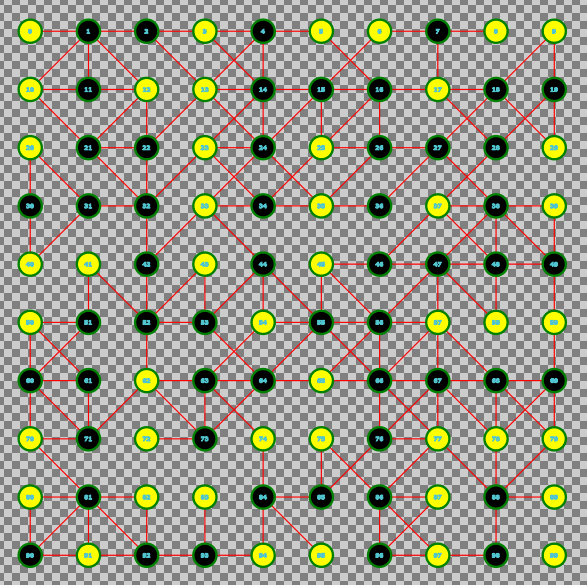
\includegraphics[scale=0.30]{/home/karly/Desktop/ACO/Doc/seed0.png}
\end{center}

Para consultar las demás semillas y replicar el experimento, basta con buscar en la carpeta GraficaSeed en dónde se muestran en formato .txt las gráficas y a su lado se encuentra el SVG de cada una de las soluciones.\\
Hay 2 archivos llamados \textbf{main.go} y \textbf{mainrandomlatiz.go} la primera corre el ejemplo del PDF que envió Luis, y la segunda versión genera las gráficas aleatoriamente, hay una parte del código que puede comentarse y ``descomentarse'' para quitar o dejar ciclos, cuando dejas los ciclos se genera par 50 gráficas diferentes y el algoritmo se ejecuta sobre las 50 diferentes gráficas y como semillas se usan los números enteros entre 0-49
ahorita como lo deje en la última versión es para que se genere una sola gráfica.

\begin{thebibliography}{Bibliografía}
 Shyong Jian Shyu, An Ant Colony Optimization Algorithm for the Minimum Weight Vertex
Cover Problem, Department of Computer Science and Information Engineering, Ming Chuan
University, 2004.
\end{thebibliography}

\end{document}

